\documentclass[border=15pt]{standalone}
\usepackage{amsmath, amssymb}
\usepackage{tikz}
\usetikzlibrary{arrows.meta}

\definecolor{block0}{HTML}{E53935}
\definecolor{block1}{HTML}{1E88E5}
\definecolor{block2}{HTML}{43A047}

\begin{document}
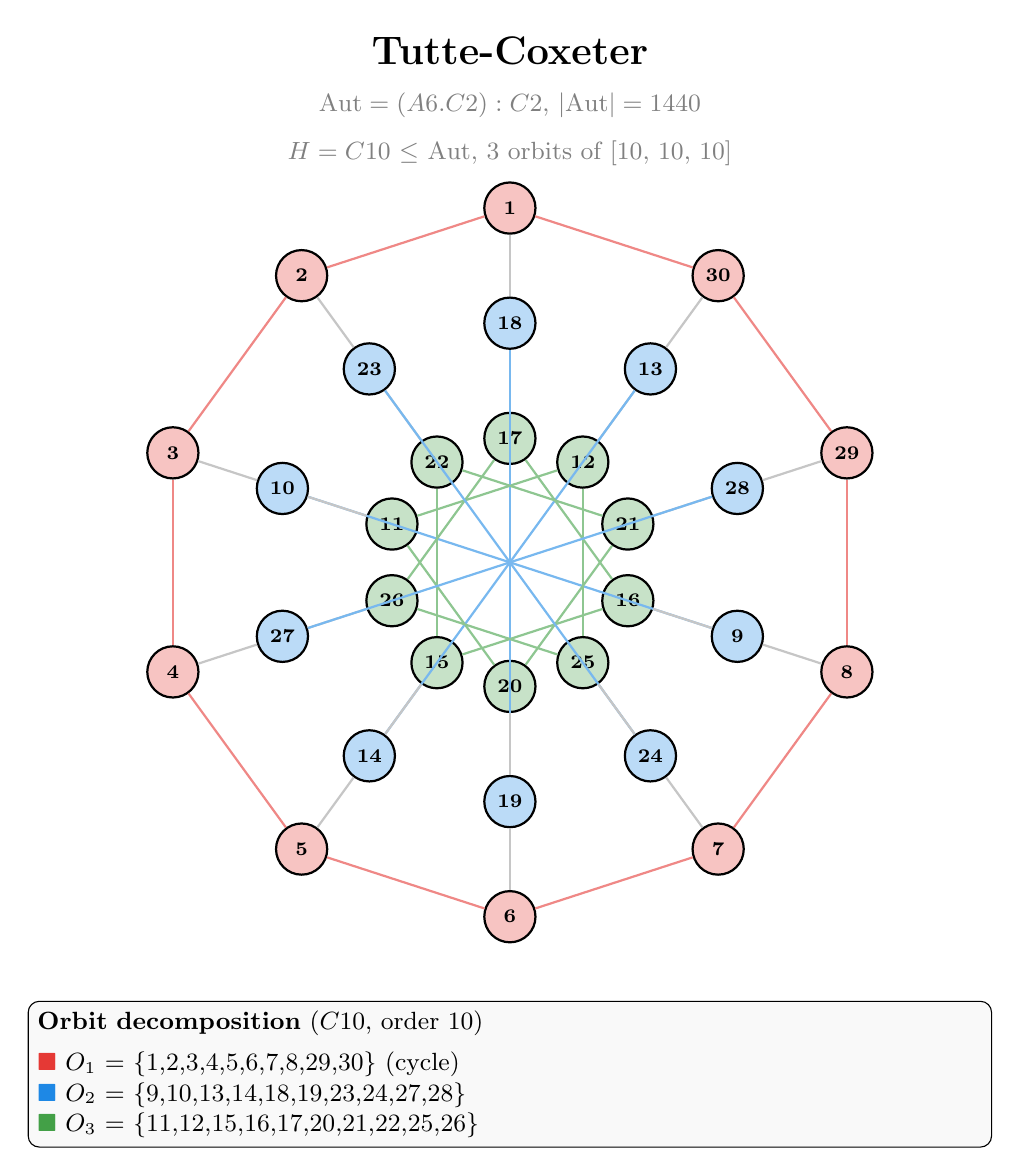
\begin{tikzpicture}[
  vertex/.style={circle, draw, thick, minimum size=6.5mm, inner sep=0pt,
                 font=\scriptsize\bfseries},
  edge/.style={thick, gray!45},
  title/.style={font=\Large\bfseries},
  subtitle/.style={font=\small, text=gray},
]

\node[title] at (0, 6.5) {Tutte-Coxeter};
\node[subtitle] at (0, 5.8) {$\mathrm{Aut} = (A6 . C2) : C2$, $|\mathrm{Aut}| = 1440$};
\node[subtitle] at (0, 5.2) {$H = C10$ $\leq$ $\mathrm{Aut}$, 3 orbits of [10, 10, 10]};

\node[vertex, fill=block0!30] (v1) at (0.000, 4.500) {1};
\node[vertex, fill=block0!30] (v2) at (-2.645, 3.641) {2};
\node[vertex, fill=block0!30] (v3) at (-4.280, 1.391) {3};
\node[vertex, fill=block0!30] (v4) at (-4.280, -1.391) {4};
\node[vertex, fill=block0!30] (v5) at (-2.645, -3.641) {5};
\node[vertex, fill=block0!30] (v6) at (-0.000, -4.500) {6};
\node[vertex, fill=block0!30] (v7) at (2.645, -3.641) {7};
\node[vertex, fill=block0!30] (v8) at (4.280, -1.391) {8};
\node[vertex, fill=block1!30] (v9) at (2.889, -0.939) {9};
\node[vertex, fill=block1!30] (v10) at (-2.889, 0.939) {10};
\node[vertex, fill=block2!30] (v11) at (-1.498, 0.487) {11};
\node[vertex, fill=block2!30] (v12) at (0.926, 1.274) {12};
\node[vertex, fill=block1!30] (v13) at (1.785, 2.457) {13};
\node[vertex, fill=block1!30] (v14) at (-1.785, -2.457) {14};
\node[vertex, fill=block2!30] (v15) at (-0.926, -1.274) {15};
\node[vertex, fill=block2!30] (v16) at (1.498, -0.487) {16};
\node[vertex, fill=block2!30] (v17) at (0.000, 1.575) {17};
\node[vertex, fill=block1!30] (v18) at (0.000, 3.038) {18};
\node[vertex, fill=block1!30] (v19) at (-0.000, -3.038) {19};
\node[vertex, fill=block2!30] (v20) at (-0.000, -1.575) {20};
\node[vertex, fill=block2!30] (v21) at (1.498, 0.487) {21};
\node[vertex, fill=block2!30] (v22) at (-0.926, 1.274) {22};
\node[vertex, fill=block1!30] (v23) at (-1.785, 2.457) {23};
\node[vertex, fill=block1!30] (v24) at (1.785, -2.457) {24};
\node[vertex, fill=block2!30] (v25) at (0.926, -1.274) {25};
\node[vertex, fill=block2!30] (v26) at (-1.498, -0.487) {26};
\node[vertex, fill=block1!30] (v27) at (-2.889, -0.939) {27};
\node[vertex, fill=block1!30] (v28) at (2.889, 0.939) {28};
\node[vertex, fill=block0!30] (v29) at (4.280, 1.391) {29};
\node[vertex, fill=block0!30] (v30) at (2.645, 3.641) {30};

\draw[thick, block0!60] (v1) -- (v2);
\draw[edge] (v1) -- (v18);
\draw[thick, block0!60] (v1) -- (v30);
\draw[thick, block0!60] (v2) -- (v3);
\draw[edge] (v2) -- (v23);
\draw[thick, block0!60] (v3) -- (v4);
\draw[edge] (v3) -- (v10);
\draw[thick, block0!60] (v4) -- (v5);
\draw[edge] (v4) -- (v27);
\draw[thick, block0!60] (v5) -- (v6);
\draw[edge] (v5) -- (v14);
\draw[thick, block0!60] (v6) -- (v7);
\draw[edge] (v6) -- (v19);
\draw[thick, block0!60] (v7) -- (v8);
\draw[edge] (v7) -- (v24);
\draw[edge] (v8) -- (v9);
\draw[thick, block0!60] (v8) -- (v29);
\draw[thick, block1!60] (v9) -- (v10);
\draw[edge] (v9) -- (v16);
\draw[edge] (v10) -- (v11);
\draw[thick, block2!60] (v11) -- (v12);
\draw[thick, block2!60] (v11) -- (v20);
\draw[edge] (v12) -- (v13);
\draw[thick, block2!60] (v12) -- (v25);
\draw[thick, block1!60] (v13) -- (v14);
\draw[edge] (v13) -- (v30);
\draw[edge] (v14) -- (v15);
\draw[thick, block2!60] (v15) -- (v16);
\draw[thick, block2!60] (v15) -- (v22);
\draw[thick, block2!60] (v16) -- (v17);
\draw[edge] (v17) -- (v18);
\draw[thick, block2!60] (v17) -- (v26);
\draw[thick, block1!60] (v18) -- (v19);
\draw[edge] (v19) -- (v20);
\draw[thick, block2!60] (v20) -- (v21);
\draw[thick, block2!60] (v21) -- (v22);
\draw[edge] (v21) -- (v28);
\draw[edge] (v22) -- (v23);
\draw[thick, block1!60] (v23) -- (v24);
\draw[edge] (v24) -- (v25);
\draw[thick, block2!60] (v25) -- (v26);
\draw[edge] (v26) -- (v27);
\draw[thick, block1!60] (v27) -- (v28);
\draw[edge] (v28) -- (v29);
\draw[thick, block0!60] (v29) -- (v30);

\node[draw, rounded corners, fill=gray!5, text width=12cm, align=left, font=\small]
  at (0, -6.5) {
  \textbf{Orbit decomposition} ($C10$, order 10) \\[4pt]
  \textcolor{block0}{$\blacksquare$} $O_{1}$ = \{1,2,3,4,5,6,7,8,29,30\} (cycle) \\
  \textcolor{block1}{$\blacksquare$} $O_{2}$ = \{9,10,13,14,18,19,23,24,27,28\} \\
  \textcolor{block2}{$\blacksquare$} $O_{3}$ = \{11,12,15,16,17,20,21,22,25,26\}
};

\end{tikzpicture}
\end{document}